\documentclass[a4paper]{report}
\setlength{\headheight}{12.0pt}
\usepackage[utf8]{inputenc}
\usepackage[T2A]{fontenc}
\usepackage[english,russian]{babel}
\usepackage[left=25mm, top=20mm, right=25mm, bottom=30mm, nohead, nofoot]{geometry}
\usepackage{amsmath,amsfonts,amssymb} % математический пакет
\usepackage{fancybox,fancyhdr}
\usepackage{xcolor}
\usepackage{hyperref}
\usepackage{tkz-euclide}
\usepackage{enumitem}
\usepackage{amsmath}
\usepackage{pgfplots}
\usepackage{float}
\usepackage{fvextra}
\usepackage[cache=false]{minted}
\usepackage[figurename=Изображение]{caption}

\hypersetup{colorlinks=true, allcolors=[RGB]{010 090 200}} % цвет ссылок
\newcommand{\lr}[1]{\left({#1}\right)} % команда для скобок
\pagestyle{fancy}
\fancyhf{}
\renewcommand{\headrulewidth}{0pt}
\fancyfoot[R]{\thepage}
\fancypagestyle{plain}{
    \fancyhf{}
    \fancyfoot[R]{\thepage}
    \renewcommand{\headrulewidth}{0pt}
}
\setcounter{page}{1} % счетчик нумерации страниц
\headsep=10mm

\makeatletter
\def\@seccntformat#1{\csname #1ignore\expandafter\endcsname\csname the#1\endcsname\quad}
\let\sectionignore\@gobbletwo
\let\latex@numberline\numberline
\def\numberline#1{\if\relax#1\relax\else\latex@numberline{#1}\fi}
\makeatother
\renewcommand{\thesection}{\arabic{section}.}
\renewcommand{\thesubsection}{\arabic{subsection}.}
\begin{document}
\subsection{Диаграмма деятельности - оформление заказа}
\begin{figure}[h]
    \centering
    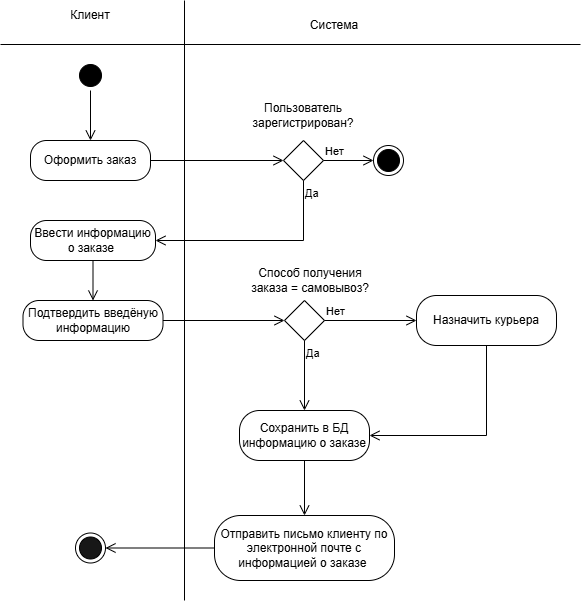
\includegraphics[width=\textwidth]{Диаграмма деятельности формирования заказа.png}
\end{figure}
$$$$\\
Предусловие: пользователь добавил в корзину как минимум один товар.\\
Пользователь перешёл к оформлению заказа. Если пользователь не зарегистрирован, то переходит к регистрации. Если пользователь зарегистрирован, то он вводит необходимую для доставки заказа информацию. Пользователь подтверждает введённую информацию. Если пользователь выбрал самовывоз, то система сохраняет информацию о заказе в БД. Если пользователь выбрал доставку курьером, то система назначает курьера для этого заказа, и сохраняет информацию о заказе и курьере в БД. Система отправляет письмо пользователю по электронной почте с информацией о заказе.\\
Постусловие: Пользователь оформил заказ\\
\newpage 
\subsection{Диаграмма деятельности - регистрация пользователя}
\begin{figure}[H]
    \centering
    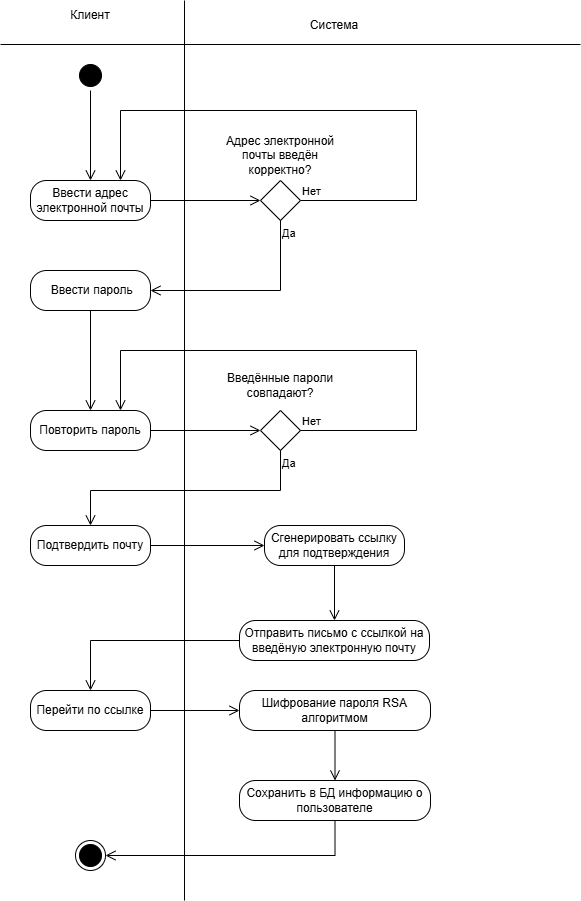
\includegraphics[width=0.85\textwidth]{Диаграмма деятельности регистрация.png}
\end{figure}
Предусловие: пользователь начал регистрацию на сайте.\\
Пользователь вводит адрес электронной почты. Если адрес электронной почты введён не корректно, то система прости ввести адрес электронной почты ещё раз. Если адрес электронной почты введён корректно, то пользователь вводит пароль. Пользователь вводит пароль повторно. Если пароли не совпадают, то пользователь вводит пароль повторно. Если пароли совпадают, то пользователь переходит к подтверждению электронной почты. Система генерирует ссылку для подтверждения электронной почты пользователя. Система отправляет письмо со ссылкой на подтверждение электронной почты по введённой электронной почте. Пользователь переходит по ссылке для подтверждения электронной почты. Система шифрует пароль пользователя RSA алгоритмом. Система сохраняет данные о пользователе в БД.\\
Постусловие: пользователь зарегистрировал аккаунт.
\subsection{Диаграмма состояний}
\begin{figure}[H]
    \centering
    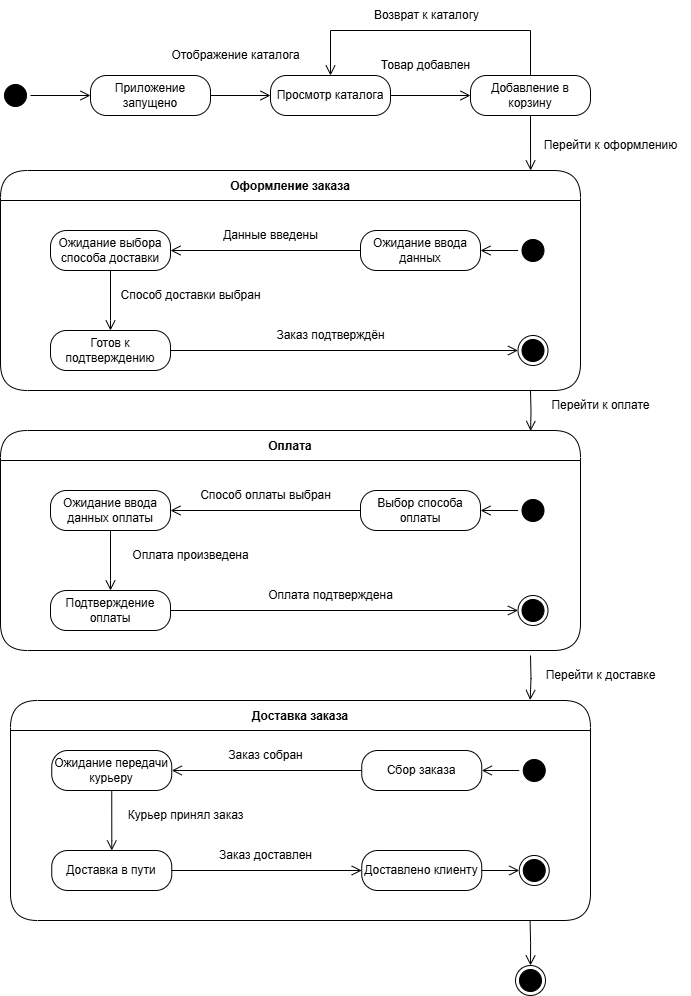
\includegraphics[width=0.85\textwidth]{Диаграмма состояний.png}
\end{figure}
Пользователь запустил приложение. Система отображает каталог товаров. В процессе просмотра каталога, пользователь добавляет товары в корзину. После чего он переходит к оформлению заказа. Система ожидает ввод данных о заказе, выбора способа доставки и подтверждения заказа. Когда данные о заказе введены, способ доставки выбран и заказ подтверждён, пользователь переходит к оплате. Система ожидает выбора способа доставки, вода данных оплаты и подтверждения оплаты. Когда выбор способа оплаты выбран, данные оплаты введены и оплата подтверждена, система переводит заказ в доставку. Начинается процесс сборки заказа, когда заказ собран он ожидает передачи курьеру. Курьер принимает заказ, после чего заказ доставляется клиенту.
\end{document}